\documentclass[10pt,aspectratio=149]{beamer}
\usecolortheme{Calm}
\usetheme{Calm}
\usepackage{pgfplots}
\usepackage{pgfplotstable}
\usepackage[utf8]{inputenc}
\usepackage{hyperref}
\RequirePackage[absolute,overlay]{textpos}
%\usepackage[sfdefault]{cabin}
%\usepackage[T1]{fontenc}
%\setlength{\TPHo{}rizModule}{\paperwidth}
%\setlength{\TPVertModule}{\paperheight}
%\definecolor{OQEdarkblue}{HTML}{046085}


\defbeamertemplate*{background canvas}{bg}
{%
  \color{lightgray!40}\vrule width\paperwidth height\paperheight% added bg color
}

%------------------------------

\author{Dominique Gravel}
\title{Research projects}
\date{August 24th, 2026}
\institute{Université de Sherbrooke \\ Summer school in biodiversity modelling}

%------------------------------
% TITLE SLIDE
%------------------------------

\usebackgroundtemplate
{
  
\includegraphics[width=\paperwidth,height=\paperheight]{bg}%
}

\begin{document}

	\begin{frame}[plain]
		\titlepage
	\end{frame}

%------------------------------

\begin{frame}{Project 1}{Metapopulation and climate change}


    \textbf{Question} : How is climate change impacting metapopulation persistence in mountainous landscapes ?

    \begin{center}
        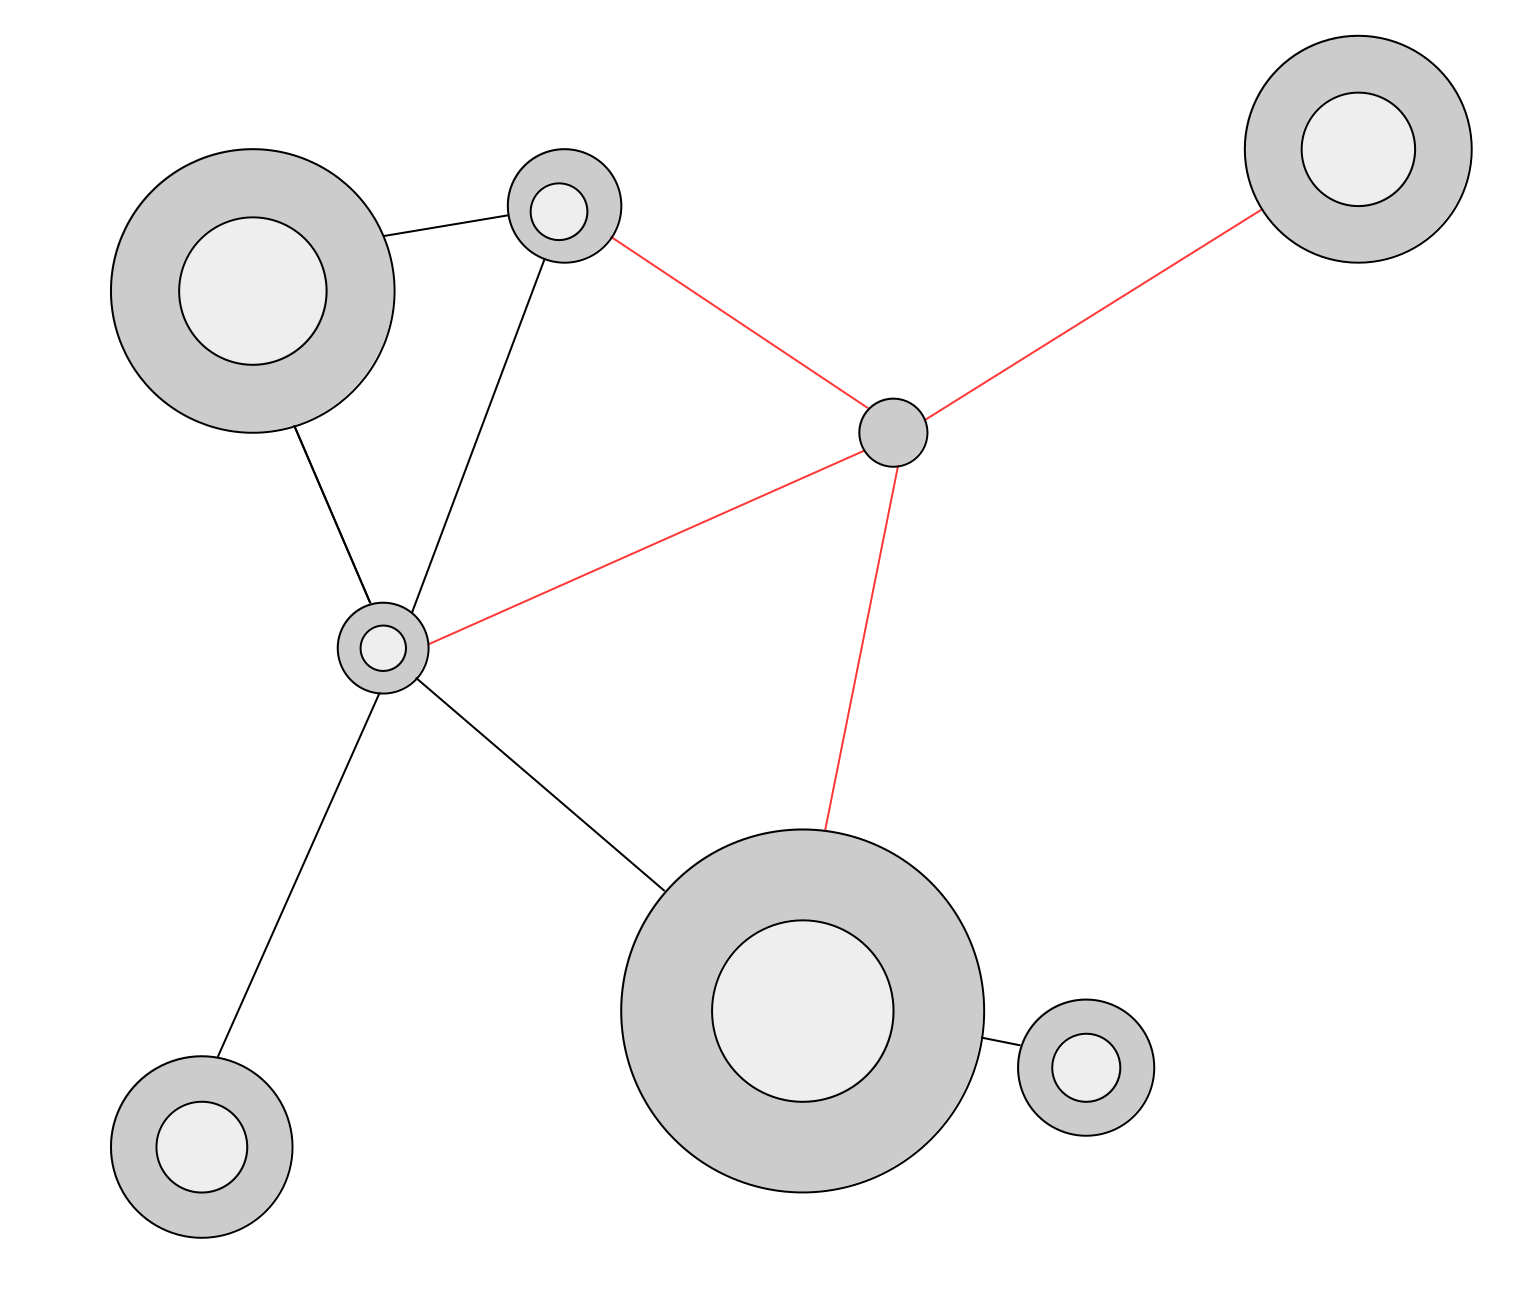
\includegraphics[height=0.7\textheight]{Figs/landscape_CC}\\
    \end{center}

\end{frame}

%------------------------------

\begin{frame}{Project 2}{Food web synchrony}


    \textbf{Question} : What is the effect of migration on the synchrony of spatial food webs ?

    \begin{center}
        
\includegraphics[height=0.7\textheight]{Figs/bylot}\\
    \end{center}

\end{frame}

%------------------------------

\begin{frame}{Project 3}{Plant-soil feedbacks}

    \textbf{Question} : How soil-plant interactions impact tree species migration at the temperate-boreal ecotone ?

    \begin{center}
        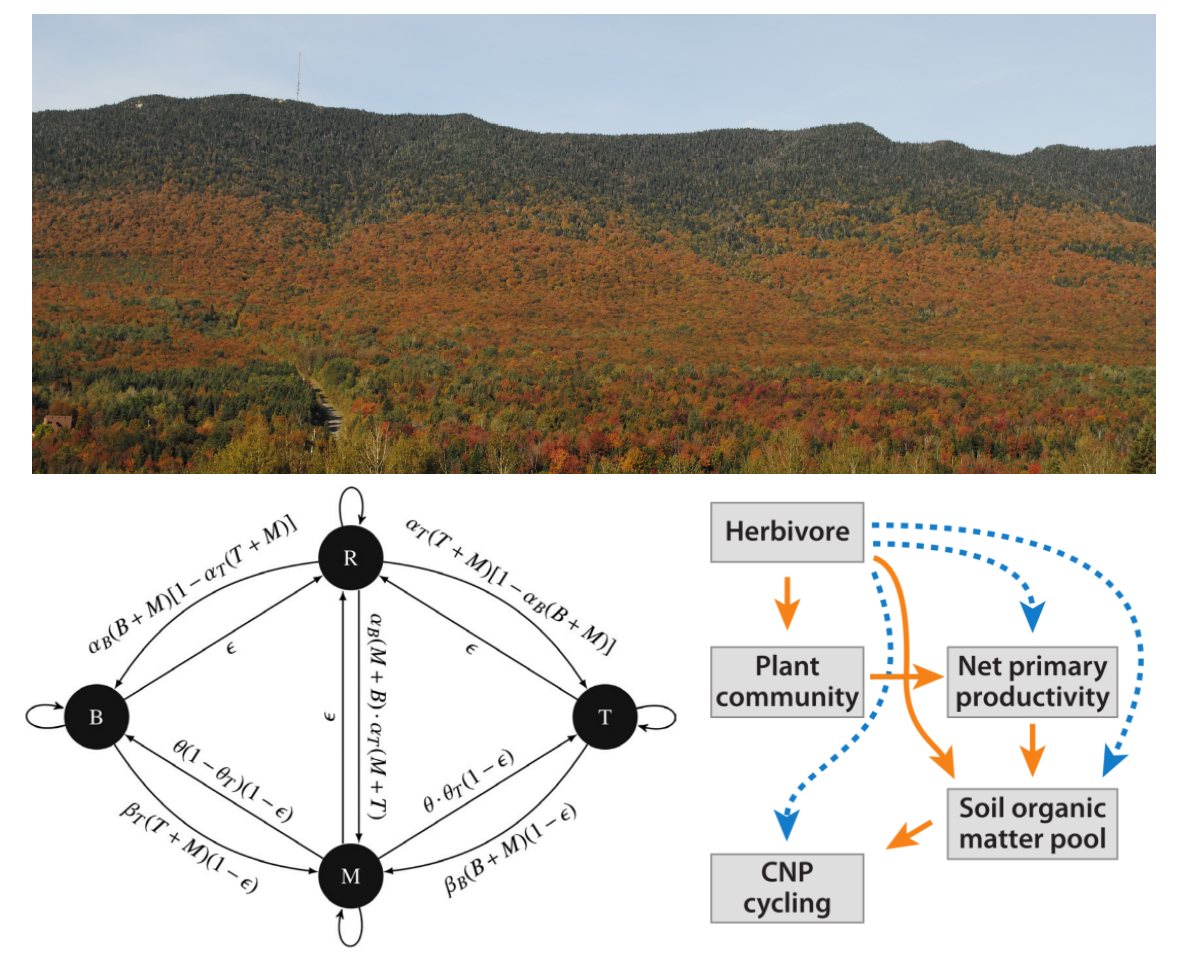
\includegraphics[height=0.7\textheight]{Figs/feedback}\\
    \end{center}

\end{frame}

%------------------------------

\begin{frame}{Project 4}{Co-occurrence}

    \textbf{Question} : What is the influence of co-occurrence on beta-diversity ?

    \begin{columns}
        \begin{column}{0.5\textwidth}							
            \begin{itemize}
                \item 200m élevation gradient
                \item 500 quadrats
                \item 10 $m^2$ plots
                \item Abundance
                \item Approx. 100 species
                \item 9 years
            \end{itemize}  
        \end{column}
%----
        \begin{column}{0.5\textwidth}
            \begin{center}
                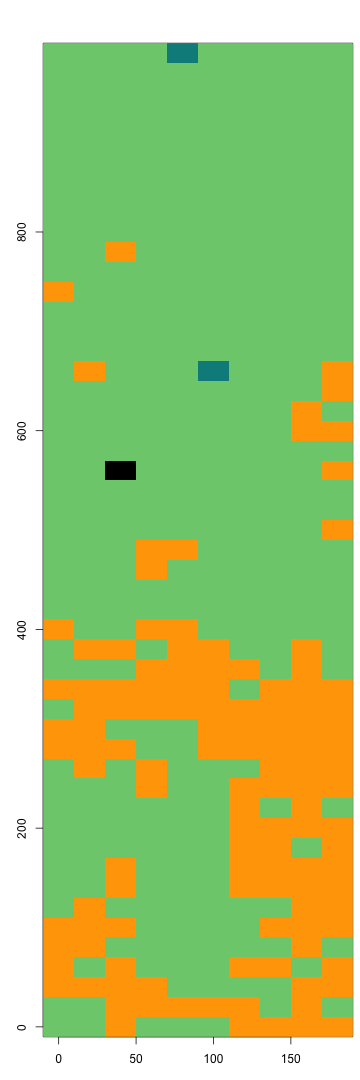
\includegraphics[height=0.6\textheight]{Figs/sutton}\\
            \end{center}
        \end{column}				
    \end{columns}

\end{frame}

%------------------------------

\begin{frame}{Project 5}{Spatial networks}

    \textbf{Question} : Are interacting species sharing the same niche ?

    \begin{columns}
        \begin{column}{0.5\textwidth}							
            \begin{itemize}
                \item Host-parasite interactions among salix, leaf gallers and paraistoids across Europe;
                \item 222 Host species;
                \item 146 Parasite species;
                \item 4 295 Interactions;
                \item 374 Locations;
                \item 32 412 species pairs; 
                \item 27 367 observed co-occurrences;
            \end{itemize}  
        \end{column}
%----
        \begin{column}{0.5\textwidth}
            \begin{center}
                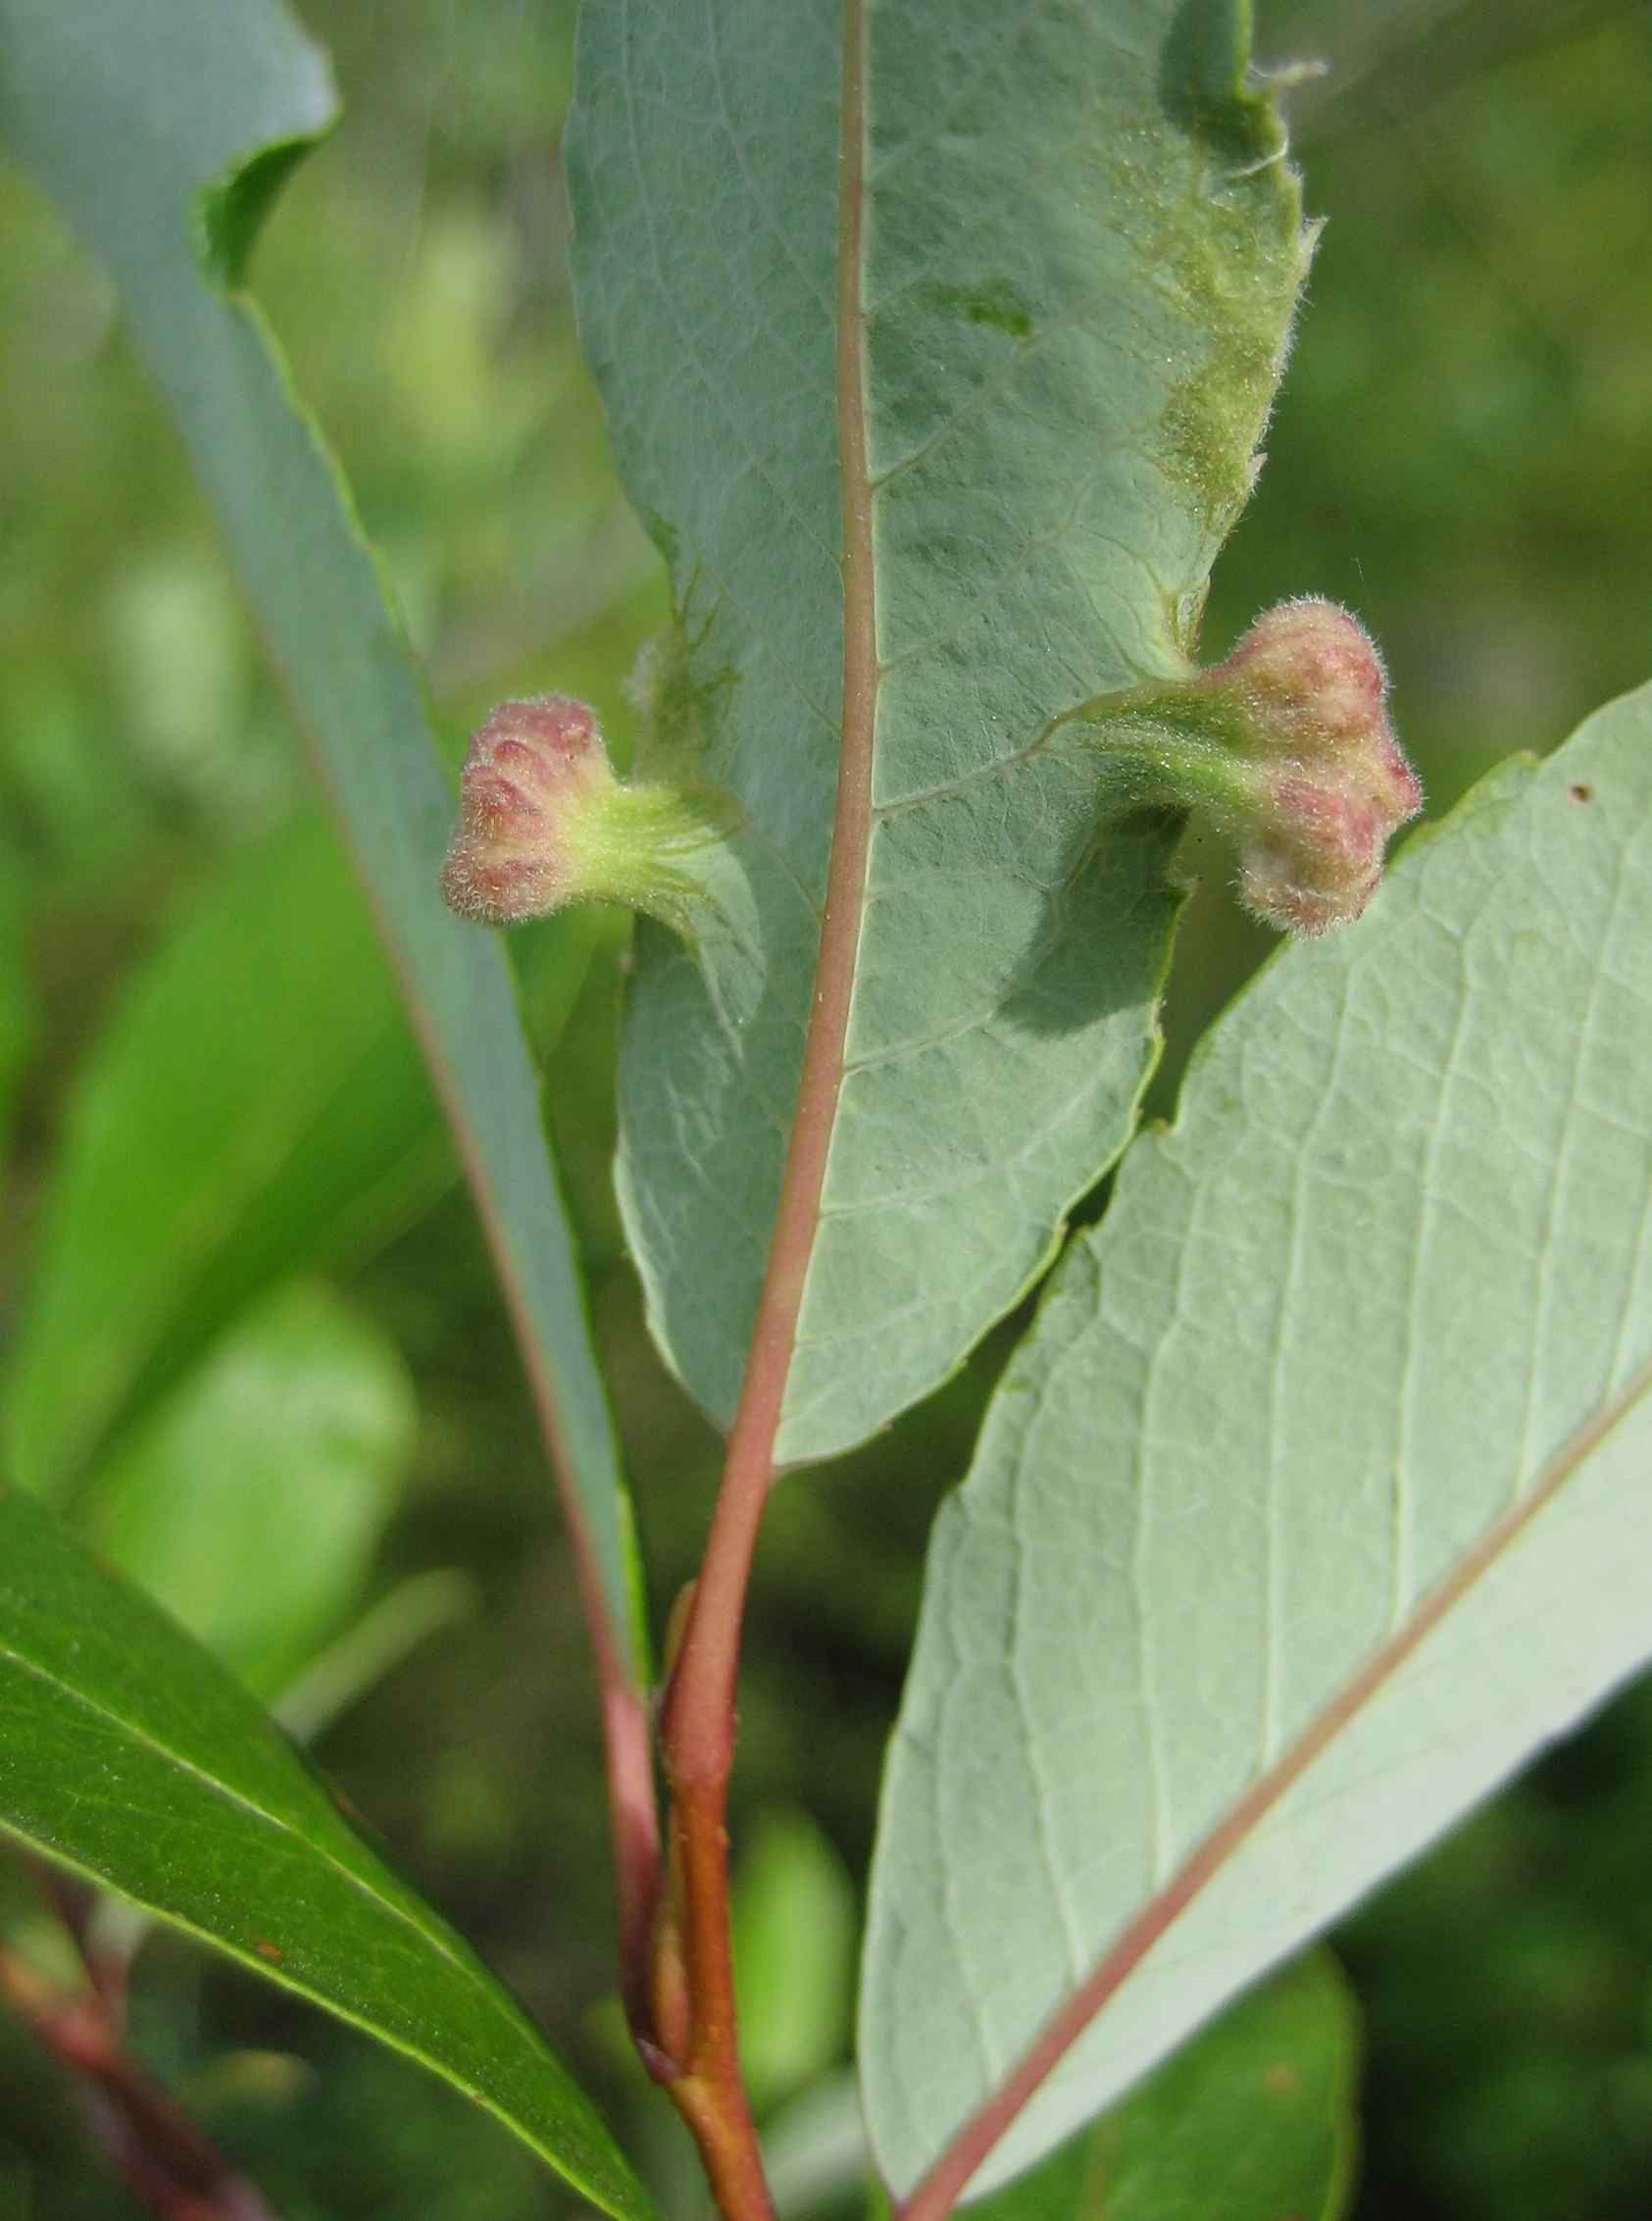
\includegraphics[height=0.6\textheight]{Figs/gall}\\
            \end{center}
        \end{column}				
    \end{columns}

\end{frame}

%------------------------------
%------------------------------
%------------------------------
%------------------------------
\end{document}
